\documentclass{report}

% Better font
\usepackage[protrusion=true,expansion=true]{microtype}
\usepackage[T1]{fontenc}
\usepackage{pxfonts}

% Misc packages
\usepackage{graphicx}
\usepackage{multirow}

% Clickable links
\usepackage{hyperref}
\hypersetup{
    colorlinks,
    citecolor=black,
    filecolor=black,
    linkcolor=black,
    urlcolor=black
}

% bibtex stuff
\usepackage{natbib}
\bibliographystyle{abbrvnat}

% Custom Commands
\newcommand{\degree}{\ensuremath{^\circ}}
\newcommand{\todo}{\textbf{TODO} }

\title{Literature Review of Point Cloud Compression}
\author{Keegan Smith\\ksmith@cs.uct.ac.za}

\begin{document}

\begin{titlepage}
\begin{center}


\includegraphics[width=100mm]{images/uct}\\
\ \\
\textsc{\Large
Department of Computer Science\\
\ \\
Honours Project Report\\
\ \\}

{\huge \bfseries
Intra-frame Compression of Molecular Dynamics Simulations of Water
\\}
\ \\
\ \\

\begin{center}
    \large Keegan Carruthers-Smith
    \\
    \small{ksmith@cs.uct.ac.za}
\end{center}

\vfill

{\large \today}

\end{center}
\end{titlepage}

% TODO citation style


\section*{Abstract}
Molecular dynamics (MD) simulations generate vast amounts of data. A typical
100-million atom MD simulation produces approximately 5 gigabytes of data per
frame consisting of atom types, coordinates and velocities.

This report surveys techniques used in point cloud compression. A point cloud
is a collection of points in 3D space. It then investigates the structure of
water. We then present a method for compressing MD data using connectivity
based point cloud compression with predictors tailored towards the structure
of water. We compare this method to more generic point cloud and data
compressors.

\todo Talk about results etc once they have been produced!

\tableofcontents

\chapter{Introduction}

Molecular dynamics (MD) simulations generate vast amounts of data. A typical
100-million atom MD simulation produces approximately 5 gigabytes of data per
frame consisting of atom types, coordinates and velocities. This will generate
17 terabytes of data a day if run for $35\,000$ steps with every 10th frame
being saved \citep{omeltchenko2000sls}. Generating this much data makes
compression desirable.

We have developed a method which compresses MD simulations. It targets
simulations which have a large amount of water in them. It uses a connectivity
based point cloud technique, but with predictors which are based on models of
the structure of water.

\todo Flesh out introduction

\chapter{Background}

% TODO Perhaps have a section to introduce new concepts near the start of the
% bg or do this as they are introduced.

% TODO Need to introduce MD format, since you refer to them later

% TODO Basic compression intro + details on entropy coding, AC,
% quantisation/dequantisation, etc. -> Some overlap with Julian

\todo update for new sections. When updating fix tense and ``we'' usage

This section introduces common techniques used in point cloud compression
algorithms, and then moves onto different categorizations and how they are
applied. We discuss how to apply these techniques to water molecule
compression. Finally, we will conclude with two general categorisations of
what the compression algorithms exploit.

\section{Point Cloud Compression}

A point cloud is a collection of point locations in 3D space. Research has
concentrated on point clouds of surfaces since point clouds are usually
generated from 3D scans of object surfaces. A surface is the ``skin'' of an
object, i.e. the boundary of a solid object.

\cite{gumholdcomp} create a tree of the points that exploit the knowledge that
the points lie on a surface. They do not, however, use predictors which
exploit this. \citet{merrycomp} extend this by using predictors which do
exploit the rectilinear nature of surface scans.

\citet{omeltchenko2000sls} compress point clouds from molecular dynamics
simulations. To exploit the density of the point clouds, a space filling curve
is created along the quantised positions. A space filling curve is one that
touches every point in a discrete space. The space filling curve used by
\citep{omeltchenko2000sls} is based on indexing the cells created by an octree
division. Then by encoding the difference between successive indicies which
contain points, they generate consistently small differences leading to good
compression rates.

\todo possibly define mesh at beginning

A mesh is a collection of vertices, edges and faces defining a 3D
object. \citet{devillers2000gci} compress meshes of 3D models. The method they
use only considers point locations, so it can be used for point cloud
compression. Their method exploits a property of kd-trees, instead of general
geometric properties.

% TODO from here to...

\section{Quantisation}

\todo need to add stuff on linear quantisation etc. Check quantisation section
in compression textbook

Point cloud data usually stores the point coordinates in a floating point
format. Most geometric compression algorithms reduce the precision to achieve
better compression rates. This reduction of precision is called
\emph{quantisation} \citep{ag-racm-03}. Every algorithm reviewed in this paper
that uses quantisation, quantises the vertex positions for each coordinate
separately and uniformly in Cartesian space. This can be visualized as
creating an evenly-spaced grid over the dimensions of the space, and snapping
the points to the closest grid point. This is the most na\"{\i}ve method, but
there are more complex methods reviewed by \citep{ag-racm-03}. These lie
outside the scope of this survey. \citet{chen2005lcp} gets around quantisation
by treating the 32-bit floating point numbers as 32-bit integers.


\section{Predictive Encoding}

Predictive compressors try to predict where a point is and then encode the
difference between its actual location and the predicted location (known as
the residual). These residuals are then encoded such that the decompressor can
calculate the point's location by the prediction added to the
residual. Entropy coding\footnote{Entropy encoding is a lossless compression
  scheme that does not exploit any characteristics of the underlying data.} is
usually applied to the encoding of residuals. If the chosen predictor(s)
exploit contextual information well, the residuals should have a low
entropy\footnote{A low entropy means we can predict what a residual will be
  well.}  leading to higher compression ratios.

% ... here is general compression stuff and should be put earlier

\subsection{Predictors}

A rooted spanning tree of the point is used in both \citep{gumholdcomp} and
\citep{merrycomp}. The creation of the spanning tree depends on what
predictor(s) are used and will be described in \ref{sec:serialization}. For
each point $v$ in the spanning tree let $v'$ be the point's parent and $v''$
be the point's grandparent.

\citet{gumholdcomp} lets the user choose between two predictors. The first is
a \emph{constant} predictor where $v$ is predicted to be at $v'$. The second
is a \emph{linear} predictor where $v$ is predicted to be at $v' + (v' -
v'')$. So either $v$ is in the same place as its parent, or it is along the
straight line $(v', v'')$ with distance $|v'-v''|$ away from its parent.

\citet{merrycomp} use the same predictors as \citep{gumholdcomp} but with two
additional predictors, the \emph{left} and \emph{right} predictors. The
surface normal\footnote{A surface normal at a point $v$ is the normal of the
  plane tangent to the surface at $v$.} $n_v$ at $v$ is heuristically
determined from $v, v'', v'$ and $n_{v'}$ (where $n_{v'}$ is the surface
normal at $v'$). From this they determine what left and right are by using the
plane determined by $n_{v'}, v'$ and $v''$. Another difference to
\citep{gumholdcomp} is that instead of letting the user choose the
predictor used, the best predictor is picked for each point. This requires the
predictor used at each point to be encoded, which is discussed next.


\subsection{Serialization}
\label{sec:serialization}

Unlike meshes, point clouds have no connectivity information. So there is no
obvious order to serialize the vertices' information (generally residuals).

\citet{gumholdcomp} create a rooted spanning tree of the points. The points
are first sorted along the $x, y$ or $z$ axis. The tree is then greedily
created by picking the first point as a root and then adding each successive
point to the vertex which minimises the residual. The tree is then serialized
by entropy encoding the out degree of each vertex in breadth-first order.

\citet{merrycomp} also create a rooted spanning tree of the points, but in a
way that favours ``long runs'' of the forward predictor. They need to encode
the predictor used at each point, so encoding the tree as \citep{gumholdcomp}
did will not work. Instead the tree is serialized by entropy coding the
predictor used in depth-first order. By favouring long runs of the forward
predictor they get better compression ratios of the encoding of the tree. To
create the spanning tree, they first create a graph of the points where every
edge with length less than $L$ is added. $L$ is the length of the longest edge
in the minimum spanning tree of the complete graph of the points. The spanning
tree is then created similarly to Prim's algorithm \citep[p.\ 457]{sedgewick},
but instead using a metric\footnote{A metric is a way to calculate the
  distance between vertices.} that favours recently considered vertices and
ones predicted well by the forward predictor.

\citet{chen2005lcp} uses a spanning tree with differential coding on the
weights. So the point cloud is encoded as a tree, with edge weights being the
difference vectors between points. They show that there exists a spanning tree
which minimises the number of pairwise different edge weights, but also show
that this is NP-Hard. They do, however, give an approximate algorithm which
uses clustering and minimum spanning trees. The tree is serialized in a simple
breadth-first order, recording the number of children for each node and the
edge weights for each child.


\section{Decoding}

When decoding the data, we may present to the user intermediate
representations of the final decompressed data as we process it. Depending on
whether we can do this or not gives us another way to classify encoders.

\paragraph{Progressive Encoder}
A progressive encoder is one that starts out streaming a coarse representation
of a point cloud. It then streams out refinements. This is useful for
transmitting the data over a network, as users can almost instantaneously see
a coarse representation. This is then followed by more and more refinements
over time as they arrive.

The use case of MD simulations require the whole file (or frame) to be
decompressed. So progressive encoders have no advantage, and are judged purely
on how well they compress the data.

\citet{devillers2000gci} provide an example of a progressive coder. The method
is best explained in 1 dimension first. If you know the total number of points
in $[a, b]$ (say $x$ points) and the number of points in $[a, (a+b)/2]$ (say
$y$ points) then the number of points in $[(a+b)/2+1, b]$ is $x - y$ . By
sending out counts of deeper and deeper levels in breadth first order they
progressively get a better representation. Encoding this with arithmetic
coding gives us the desired compression ratios. To extend to 3 dimensions one
uses a process similiar to creating a kd-tree: at each step subdivide along a
different dimension.

\paragraph{Single-Rate Encoding}
A single-rate encoder is one which requires the whole stream to be available
before the data can be decompressed. \citet{omeltchenko2000sls},
\citet{gumholdcomp} and \citet{merrycomp} are all single-rate encoders.


\section{Modelling Water}

\todo references

\begin{figure}[h]
\centering
\resizebox{0.75\textwidth}{!}{
  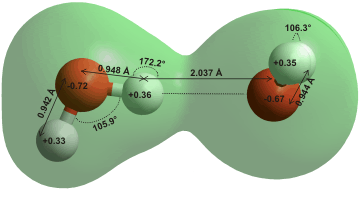
\includegraphics{images/h402}
}
\caption{The most energetically favourable water dimer calculated from first
  principles.}
\label{fig:dimer}
\end{figure}

\begin{figure}[h]
\centering
\resizebox{0.5\textwidth}{!}{
  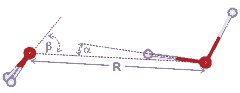
\includegraphics{images/dimr}
}
\caption{Water dimer angles. $R = 2.976\AA, \alpha = 6 \pm 20\degree, \beta =
  57 \pm 10\degree$}
\label{fig:dimer-angle}
\end{figure}

The previously discussed predictors work well in the setting of general point
clouds, but in a point cloud consisting of water molecules we can create
predictors tailored towards water.

A water dimer is two water molecules loosely bonded by a hydrogen atom. This
is the simplest model for hydrogen bonding in water, and as such has been
extensively studied.

The oxygen which is loosely bonded to the hydrogen is expected to be
$2.976\AA$ away from the other oxygen. It is also expected that the vector
created by the O-H bond to be roughly in line with the vector of the loose O-H
bond. See Figure \ref{fig:dimer} and Figure \ref{fig:dimer-angle}.

\subsection{Using the Model in Point Cloud Compressors}

\todo should this be in the design chapter?

\citet{omeltchenko2000sls} only exploit the fact that we have many dense
clusters in MD simulations. It is more general than water compression, and
modifying it to use the relative layouts of the water molecules is not clear.

The predictors of \citet{merrycomp} and \citet{gumholdcomp} do not exploit the
layout of water molecules. Using water dimer model prediction can be done
given the positions of a water molecules atoms. The creation of the spanning
tree would be different, since we know the expected degree of the verticies is
at most two.

\begin{table}[t]
\centering
\resizebox{\textwidth}{!}{
\begin{tabular}{||l|c|c||}
  \hline
  \emph{Attribute/Method} & \citet{omeltchenko2000sls} & \citet{gumholdcomp} \\

  \hline

  \emph{Structure} & MD Simulation & Surface \\

  \emph{Progressive} & Single-rate & Single-rate \\

  \emph{Quantisation} & Yes & Yes \\

  \emph{Connectivity} & Space Filling Curve & Spanning Tree \\

  \emph{Exploits} & Dense/regular clusters & Regularity of scans \\

  \emph{Scope} & Global & Local \\

  \emph{Topology} & Geometry & Both \\

  \hline
  \hline

  \emph{Attribute/Method} & \citet{chen2005lcp} & \citet{devillers2000gci} \\

  \hline

  \emph{Structure} & 3D Model & Mesh \\

  \emph{Progressive} & Single-rate & Progressive \\

  \emph{Quantisation} & No & Yes \\

  \emph{Connectivity} & Spanning Tree & kd-trees \\

  \emph{Exploits} & Differential Coding & kd-tree properties \\

  \emph{Scope} & Global & Global \\

  \emph{Topology} & Connectivity & Neither \\

  \hline
  \hline

  \emph{Attribute/Method} & \citet{merrycomp} & \\

  \hline

  \emph{Structure} & Surface & \\

  \emph{Progressive} & Single-rate & \\

  \emph{Quantisation} & Yes & \\

  \emph{Connectivity} & Spanning Tree & \\

  \emph{Exploits} & Rectilinear scans & \\

  \emph{Scope} & Local & \\

  \emph{Topology} & Both & \\

  \hline
\end{tabular}
}
\caption{Taxonomy of the different methods.}\label{tab:taxonomy}
\end{table}


\section{Taxonomy of Techniques}

Refer to Figure \ref{tab:taxonomy} for an overview of the categorisations of
the different papers. There are two underlying philosophies which the
compression algorithms exploit, the \emph{scope} and the \emph{topology}.

\emph{Scope} is whether the algorithm is exploiting \emph{global} or
\emph{local} properties of the points. \citet{merrycomp} uses a local scope
since it exploits nearby points to predict the location of the current
point. \citet{chen2005lcp} uses a global scope, since it is trying to minimise
a global property of the spanning tree.

\emph{Topology} is whether the algorithm is trying to exploit connectivity or
geometric information. \citet{gumholdcomp} exploits both, but the geometry
more since it uses a predictor to predict the location based on other points
location. \citet{chen2005lcp} just tries to choose the best possible spanning
tree, so they exploit connectivity of points.

The other properties listed in the taxonomy are \emph{structure},
\emph{progressive}, \emph{quantisation}, \emph{connectivity} and
\emph{exploits}.

\begin{itemize}
\item \emph{Structure} is what type of point cloud the compressor targeting.

\item \emph{Progressive} is whether the compressor is a single-rate encoder or
  progressive encoder.

\item \emph{Quantisation} is whether the compressor applies quantisation
  before compression.

\item \emph{Connectivity} is how relationships between points are derived or
  modelled.

\item \emph{Exploits} is what the compressor is targeting for good
  compression.
\end{itemize}


\section{Summary}

The water dimer model gives a good predictor for exploiting the local
structure of water molecules. So using a predictive point cloud encoder
similiar to \citep{merrycomp} and \citep{gumholdcomp} should result in good
compression of water molecules.

Compressing the other atoms will require a more general technique. Using the
best point cloud compressor on the other atoms combined with the water
prediction scheme should result in better compression.


\chapter{Design and Implementation}

\todo Need to justify decisions, not just list them! \\

This chapter outlines the design of our compressor and decompressor. The
compression techniques investigated only cover intra-frame
compression\footnote{Intra-frame compression is where we compress each frame
  independently of the other frames.}, but our final product handles
multiframe compression and visualisation as well. As such the design needs to
take into account these uses, but components outside of the scope of
intra-frame compression will not be covered.

\section{Overview}

Compression is done on the DCD/PDB format, which is a format for storing MD
simulations. DCD files are readable by VMD. \todo references.

A high-level overview of how data flows in the compressors is illustrated by
the following: \todo replace with pretty picture similiar to the FBI
fingerprint compression paper

\[ DCDFile \to Atoms \to QuantisedAtoms \to Compressor \]

The decompressor works in the reverse direction:

\[ Decompressor \to QuantisedAtoms \to DCDFile \]

The decompressed DCD files have been quantised. Excluding the quantisation
step, the scheme is lossless. Note that each step in the compression phase has
auxillary information. The auxillary information is required for
reconstruction.

Reference implementations of \citep{devillers2000gci}, \citep{gumholdcomp} and
\citep{omeltchenko2000sls} where also created. These use the DCD I/O to read
in the MD simulation files. Julian Kenwood implemented
\citep{omeltchenko2000sls}, while Keegan Carruthers-Smith implemented
\citep{devillers2000gci} and \citep{gumholdcomp}.


\subsection{Dependencies}

\todo Implementation chapter \\

All development was done on Linux, but no Linux or POSIX specific APIs where
used. So the implementation should be cross platform barring library
dependencies which are not.

\todo References

\paragraph{C++}
C++ fits the requirements of this project since compressors need to be fast
and all the authors are competent with it. Development was done with GCC 4.x.

\paragraph{ANN}
ANN is a library for approximate nearest neighbor searching. It is used to
speed up graph creation where locality of points is important.

\paragraph{VMD DCD Loader Plugin}
This plugin is used to read and write DCD files.


\section{Components}

A component-based approach was used to design the compressor and
decompressor. This is because the algorithm can be broken up into distinct
steps.

\todo picture showing components and who did what

The different components are the following:

\paragraph{Simulation I/O}

These components handle I/O to and from the files we are compressing. We are
compressing DCD files. DCD files come with accompanying PDB file, which
contains info about what each atom is in the DCD file.


\paragraph{Arithmetic Coder}

The ``meat'' of all the compression schemes convert the input into a symbol
stream (where the symbols are from a fixed alphabet). These symbols are then
compressed with an arithmetic encoder. Similarly the decompressor takes a
symbol stream and converts it into the original input.

The arithmetic coder has two parts to it, a \emph{reader} and a
\emph{writer}. The \emph{reader} and the \emph{writer} are inverses to each
other, with the \emph{reader} converting a symbol stream to a bit stream and
the \emph{writer} converting a bit stream to a symbol stream.

The encoder by \citep{omeltchenko2000sls} does not make use of an Arithmetic
Coder, instead it uses its own coder. Every other encoder uses the arithmetic
encoder.


\paragraph{Quantiser}

The quantiser is responsible for quantising and dequantising a frame. A frame
is a collection of points in three dimensional space. Each coordinate of the
point is specified as a floating point value. The quantiser takes in as input
a number $b$. It then converts each floating point value to a $b$-bit integer.

Converting the floating point value to an integer introduces error. This is
the only step which is lossy. It is necessary to quantise since we need the
prediction residuals to be small and common. Without quantisation the
residuals will be close, but not the same. This leads poorer compression.

\todo what a frame is should be explained in background.


\paragraph{Permutations}

When decompressing we need to recover the atoms in the same order they are
listed in the original DCD file. How we recover the order is explained in
Section \ref{sec:compr-perm}.


\paragraph{Compressors}

The compressor component is different for each compressor. There is the
compressor presented in this report and the three reference compressors:
\citet{omeltchenko2000sls}, \citet{gumholdcomp} and \citet{devillers2000gci}.


\section{Water Compressor}

This section details the algorithm of the water compressor and is the main
contribution of this report. This algorithm is implemented as a compressor
component and uses the components detailed in the last section.

The compressor processes each quantised frame in order. This algorithm is an
intra-frame compressor, and as such only compresses using information
contained in the frame.

The algorithm is similiar to the predictive point cloud compressors of
\citep{gumholdcomp} and \citep{merrycomp}. The following is a high level
overview of the algorithm:

\begin{verbatim}
CompressFrame(list_of_atoms_in_frame, arithmetic_encoder):
  list_of_water_molecules = FindWater(list_of_atoms_in_frame)
  list_of_other_atoms = FindNonWater(list_of_atoms_in_frame)
  compress(list_of_other_atoms, arithmetic_encoder)
  water_graph = CreateGraph(list_of_water_molecules)
  spanning_tree = CreateSpanningTree(water_graph)
  TreeSerialise(spanning_tree, arithmetic_encoder)
\end{verbatim}

\noindent Similarly decompression uses this algorithm:

\begin{verbatim}
DecompressFrame(arithmetic_decoder):
  list_of_other_atoms = decompress(arithmetic_decoder)
  list_of_water_atoms = TreeDeserialise(arithmetic_decoder)
  return list_of_other_atoms + list_of_water_atoms
\end{verbatim}

\todo once we get more substantial results we can pick which point cloud compressor to use

Each part of the high level overview is explained in the rest of this section.


\subsection{Finding Water Molecules}

The PDB file associated with a DCD file contains information on which atoms a
given atom is bonded to. Using the PDB file we find all oxygen atoms which are
bonded to two hydrogen atoms. This section was implemented in the Simulation
I/O component.


\subsection{Water Predictors}

The predictors are based on the models of water dimers explained in the
background chapter. There are three predictors used, the constant predictor
and the two hydrogen predictors.

Let $O, H_1, H_2$ be the predictions for where the water molecule will be and
let $O', H'_1, H'_2$ be the water molecules parent.

\paragraph{Constant Predictor}
The constant predictor predicts $O, H_1, H_2$ to be at $O'$.

\paragraph{Hydrogen Predictor}
The hydrogen predictor predicts along $O'-H'_1$ or $O'-H'_2$. We simplify the
model in Figure \ref{fig:dimer-angle} and assume $\alpha$ is $0\degree$. We
predict $O$ to be at $O' + 2.976\frac{O'-H'_i}{|O'-H'_i|}$. Due to the large
variability of $\beta$ in Figure \ref{fig:dimer-angle} we predict $H_1$ and
$H_2$ to be at $O$ in both predictors.


\subsection{Creating the Water Graph}

A directed graph is created of the water molecules. The water molecules are
the verticies of the graph. There is an edge from $O$ to $O'$ if $O'$ is a
candidate for good prediction from $O$.

The graph is created iteratively. There is an edge between two water molecules
if their respective oxygen atoms are within $3\AA$. Due to the forces involved
the number of oxygen atoms within $3\AA$ is small. Na\"{\i}vely this takes
$O(N)$ where $N$ is the number of water molecules. To speed this up a kd-tree
is created of the molecules. A molecule's position is the position of its
oxygen atom. Using the kd-tree the search takes approximately $O(\log(N))$
where $N$ is the number of water molecules. This is done per molecule so the
overall complexity of graph creation is $O(N\log(N))$.


\subsection{Creating the Spanning Tree}

\todo needs psuedocode

\todo this explains the current method. improvements: do a MST to connect
forest. Be less greedy with predictions, don't encode everything it is
connected to. Maybe use dijkstra modification instead of a BFS

This stage takes the graph and creates a directed spanning tree. Each edge
indicates which predictor is used.

The graph is not necessarily connected, so a tree is created for each
component. A root vertex is arbitrarily selected. Then each tree in the forest
is connected to it with the constant predictor. The serialiser needs to know
what the root is.

For each component a root is arbitrarily picked. Then a BFS starts at the
root. For each vertex every unseen vertex is greedily assigned the predictor
which gives the smallest residual. The unseen vertex is then set to seen and
added to the queue. When the queue is empty every vertex in the component has
been visited.


\subsection{Tree Serialisation}

\todo This section needs a lot of improvement

This stage writes the spanning tree to the file. It encodes the spanning tree
in BFS order starting at the root. For each water molecule it does the following:

\begin{verbatim}
predictions = get_predictions(water_molecule)
errors = water_molecule.positions - predictions
error_encoder.encode(errors)

permutation_encoder.encode(water_molecule.index)

for child in water_molecule.children_verticies:
  child.parent = water_molecule
  tree_encoder.encode(child.predictor)
  bfs_queue.push(child)
tree_encoder.encode(end of children sentinal)
\end{verbatim}


\subsection{Tree Deserialisation}

\todo

\chapter{Random sections to be integrated properly}

\section{Compressing Permutations}
\label{sec:compr-perm}

Every compression algorithm explored in this report does not necessarily
preserve the order of the points when decompressed. For example in
\cite{devillers2000gci}
\[ (1, 2), (1, 3), (0, 0), (2, 3), (2, 2), (0, 2), (1, 1) \]
when decompressed becomes
\[ (0, 0), (1, 1), (0, 2), (1, 2), (1, 3), (2, 2), (2, 3) \]

When decompressing we need to recover the original order of the points, since
the index of a point indicates which atom it is in the DCD file format.

We experimented with five different types of permutation compressors. Each
permutation compressor takes in a permutation of $[0,1,\dots,N-1]$ and writes
it to the file. Let the permutation be $[P_0, P_1, \dots P_{N-1}]$.  The
decompressor then recovers the permutation.

\paragraph{Null}
Null does not write anything to the file. The decompressor just outputs the
order permutation $[0,1,\dots,N-1]$. A compressor which uses the null
compressor does not preserve the order. Every other permutation compressor
should do worse than this.

\paragraph{Na\"{\i}ve}
Na\"{\i}ve writes the permutation list straight to the file. Each index is
stored as a $32$-bit integer. Every other permutation compressor should do
better than this.

\paragraph{Delta}
Delta transforms the permutation into a list $L$, where $L_0 = P_0$ and $L_i =
P_i - P_{i-1}$ for $0 < i < N$. Arithmetic encoding is then done on $L$. $L$
is then written to file.

Decompression gets back the list $L$. Since $P_0 = L_0$ and $P_i = L_i +
P_{i-1}$ for $0 < i < N$ we can recover the original permutation. Since each
$P_i$ depends only on previous $i$'s, calculating $P_i$ in increasing order of
$i$ will recover $P$.

\paragraph{Interframe}
Interframe transforms the permutation $P$ into a list $L$. Let $P'$ be the
permutation from the previous frame. If it is the first frame, let $P' =
[0,1,\dots,N-1]$. Then $L_i = P_i - P'_i$ for $0 \le i < N$. Use arithmetic
encoding on $L$ and then write $L$ to file.

Decompression recovers the list $L$. Since $P_i = L_i + P'_i$, $P$ can be
recovered. Note that this method requires frames to be decompressed in order.

\paragraph{Optimal}
Optimal uses a static arithmetic coder with a frequency of $1$ for each
$P_i$. Since each $P_i$ occurs only once, this gives the best possible
compression.

A static arithmetic encoder model uses a Fenwick Tree to update the symbol
table after each encoding. This takes $O(\log(N))$ per update. In the optimal
permutation compressor we can get this down to $O(1)$ by using the fact that
we only ever encode each $P_i$ once. To encode a symbol $i$ the arithmetic
encoder requires $S_{tot}$, $S_i$ and $S_{i-1}$. $S_{tot}$ is the sum of all
the frequencies. $S_i$ is the sum of the frequencies for all the symbols less
than or equal to $i$. Since the frequency of each index is one, $S_i = i$ and
$S_{tot}$ is the number of permutations left. We need a way to map permutation
indicies to symbols which is quick to update once an index has been
encoded. The following algorithm is used:

\begin{verbatim}
init(permutation):
  number_of_symbols = permutation.size
  for i in 0, 1, ..., permutation.size - 1:
    index_to_symbol[i] = i
    symbol_to_index[i] = i
\end{verbatim}

\begin{verbatim}
pop_index(index):
  number_of_symbols--

  symbol = index_to_symbol[index]
  index2 = symbol_to_index[number_of_symbols]

  index_to_symbol[index2] = symbol;
  symbol_to_index[symbol] = index2;

  return symbol;
\end{verbatim}

\begin{verbatim}
pop_symbol(symbol):
  index = symbol_to_index[symbol]
  pop_index(index)
  return index
\end{verbatim}

Then to encode $P_i$, we encode $pop\_index(P_i)$. To decode, we use
$pop\_symbol(decoded\_val)$.

\section{Verifiers}

Once a DCD file has been compressed and then decompressed we have a DCD file
approximating the original DCD file. The compressor is expected to be lossless
once quantisation has occurred. So to verify a compressor on a DCD file the
following process is done:

\begin{verbatim}
Verify(Compressor comp, Quantiser quant, DCD dcd):
  dcd_quant1 = quant.quantise(dcd)
  dcd_quant2 = comp.decompress(comp.compress(dcd_quant1))
  return dcd_quant1 == dcd_quant2
\end{verbatim}

Note that \emph{quant.dequantise(dcd\_quant2)} will not likely be equal to
\emph{dcd}. This is because the quantisation stage is lossy.

\nocite{*}
\bibliography{report_keegan}

\end{document}
